\documentclass[12pt]{article}
\usepackage{graphicx}
\usepackage{listings}
\usepackage{fullpage}
\usepackage{tikz}
\usepackage{enumitem}
\usepackage{pdfpages}
\usetikzlibrary{shapes,arrows,calc,automata}

\lstset{ %
language=Java,
basicstyle=\small \ttfamily,commentstyle=\scriptsize\itshape,showstringspaces=false,breaklines=true,numbers=left}

\usepackage{fontspec}
\setmonofont{Cousine}[Scale=MatchLowercase]

\begin{document}

\title{Software Testing, Quality Assurance \& Maintenance (ECE453/CS447/SE465): Final}
\author{}
\renewcommand{\today}{}
\maketitle

 ~\\[-7em]

\begin{center}
{\Large April 21, 2017}
\end{center}

This open-book midterm has 7 questions, each worth 20 points. Answer the
questions in your answer book. You may consult any printed material
(books, notes, etc).


\section*{Question 1. Short Answer}
Which tool could you use to find the following problems? {\bf Name the tool} and {\bf describe} which class of techniques it belongs to. Also {\bf name a limitation of/challenge for} that tool/technique in that situation.
{\bf Write} one or two sentences for each situation.

[Example: ``race conditions'': Helgrind. This \emph{dynamic analysis
    tool} looks for a write to memory that occurs concurrently with a
  read of the same location with no common locks between the read or
  the write. Dynamic analysis only detects problems on code paths that
  get executed.]

\begin{enumerate}[label=\alph*.]
\item program does not conform to project style guides forbidding use of global variables.
\item program is accessing memory outside array bounds.
\item variable names don't describe their contents.
\item program is difficult to use (not user-friendly).
\item developers commit source to shared repository that fails to compile on machines other than their own.
\end{enumerate}

\section*{Question 2: Code Review}
Consider the Java code in {\tt SourceFileScope}, attached. {\bf Review} 3 aspects of the code. {\bf Explain} each aspect in a couple of
sentences, supporting it with examples from the code that you're
reviewing. 

\includepdf[pages=-,pagecommand={},width=1.1\textwidth]{SourceFileScope.pdf}

\section*{Question 3: Mock Objects}
You are given the following code that represents a one dimensional world with transportation, with distances measured as integer kilometers and prices measured as integers.

\begin{lstlisting}
interface Transport {
    Vehicle hailVehicle();
    int getPricePerKm();
}

interface Vehicle {
    Driver getDriver();
    void waitUntilArrivedAt(int location);
}

interface Driver {
    void setDestination(int location);
    void pay(int amount);
}

interface Wallet {
    Wallet(int initialAmount);

    void takeOut( int amount ) throws YouAreBrokeException;
    int getAmount();
}

class Person {
    Person( int home, int currentLocation, Wallet wallet ) { /* init fields */ }

    Wallet wallet; Wallet getWallet() { return wallet; }
    int home; int getHome() { return home; }
    int location; int getLocation() { return location; }

    void goHomeUsing(Transport t) {
        Vehicle v = t.hailVehicle();
        v.getDriver().setDestination( getLocation() );
        v.waitUntilArrivedAt( getHome() );

        int payment = t.getPricePerKm() * Math.abs(getHome() - getLocation());
        getWallet().takeOut( payment );
        v.getDriver().pay( payment );
    }
}
\end{lstlisting}

The following is what your colleague implements to test the Passenger.goHome() method using mocking. Assume that these mocks throw an exception---i.e. fail the test---if any unexpected calls are made. Also assume that the order doesn't matter.

\begin{lstlisting}
@Test
void testGoHome() {
    Transport   mockTransport   = mock(Transport);
    Vehicle     mockCar         = mock(Vehicle);
    Driver      mockDriver      = mock(Driver);

    // Tells our Transport interface to return our mocked Vehicle instead.
    mockTransport.hailVehicle().andReturn(mockCar);

    // Like above...except for Driver and we allow it to be called
    // as many times as the dev desires.
    mockCar.getDriver().anyTimes().andReturn(mockDriver);

    mockDriver.setDestination( 5 );
    mockTransport.getPricePerKm().anyTimes().andReturn( 1 );
    mockDriver.pay( 10 );

    // Done setting expectations.
    replayAll();

    // Testing...
    Person  patrick = new Person( 5, 100, new Wallet(500) );
    patrick.goHomeUsing( new UberTransport() );

    // Verify our expectations were met.
    verifyAll();
}
\end{lstlisting}
{\bf Part a.} There are 3 mistakes in the above test. (A mistake causes the test case to not
encode/verify the behaviour of the actual {\tt Person} class.) {\bf Identify} and {\bf fix} them.

\noindent
{\bf Part b.} Your colleague then mentions that they forgot to add an assert to the test and, with haste, appends
\begin{lstlisting}[numbers=none]
    assertTrue( patrick.getWallet().getAmount() == 405 );
\end{lstlisting}
to the end of the test. {\bf Explain} why this is inconsistent and propose a change to the test code that utilizes mocking instead.

\section*{Question 4: Finite State Machines}
Consider a candy dispensing machine that can either output Snarties or N\&Ns.
Possible input actions are:
\begin{itemize}[noitemsep]
\item insert money (let's assume the input is \$1, one coin only);
\item select Snarties;
\item select N\&Ns;
\item cancel operation.
\end{itemize}
Once the machine has received both the money and the choice of candy
(in either order), it performs the output action, ``dispense
candy'', and returns to the initial state. The cancel button may trigger the ``refund money'' output
action.

{\bf Draw} a Finite State Machine which summarizes the potential behaviours
of this machine; edges should be labelled with input actions and
output actions (when appropriate). {\bf Write down} a minimal test set (smallest total \# of actions) that achieves
Simple Round Trip Coverage. {\bf Write down} a test set that achieves
Complete Round Trip Coverage.

\section*{Question 5: Selenium}
Imagine the following situation: Your task is to go through a list of
88 search results on a webpage. For each of the results, you need to
visit the link, enter a value on the resulting page, and hit save. (You find yourself
wondering which of your poor life choices resulted in this
situation\footnote{This scenario is not imaginary, but it is simplified.}.)

You remember that you heard something about Selenium, which allows you
to automate web interactions (or run tests). You attempt to record the
required interaction, and you get the following XPath query as part of your result.

\begin{center}
  \verb+xpath=(//input[@id=dp1492644142915])+
\end{center}

Regrettably, you find your macro does not generalize to other search
results. {\bf Explain why.}

You open the relevant input field in Firebug and find the following HTML:
\begin{lstlisting}
<td class="label">
  <label for="custom_1_170">Board approval date</label>
</td>
<td class="html-adjust">
  <input id="custom_1_170" class="crm-form-text crm-hidden-date"
         data-crm-custom="OAC_Regular_Membership_fields:Board_approval_date"
         type="text">
  <input id="dp1492644142915" class="crm-form-text crm-form-date hasDatepicker valid"
         type="text" aria-invalid="false">
\end{lstlisting}
{\bf Write down} an XPath query that will select the same input field as above, but that will
also work across different search results. Include the assumptions that you are making to
support your answer.

After using your macro a few times, you notice that it is flaky and
sometimes fails to select the desired input. Assume that your macro is correct.
{\bf Explain} why your macro is flaky. Also {\bf explain} how you can fix the macro to mitigate the failure.

\section*{Question 6: Coverage}
Consider the following code:
\begin{lstlisting}[numbers=none]
  class TreeNode {
    int data;
    TreeNode left, right;
  }

  void traverse(TreeNode n, List<Direction> choices) {
    TreeNode cur = n;             // line A
    for (Direction d : choices) { // line B
      print (cur.data % 2);       // line C
      switch (d) {                // line D
        case Direction.LEFT:
          cur = cur.left; break;  // line E
        case Direction.RIGHT:
          cur = cur.right; break; // line F
      }
    }
    print (cur.data % 2);       // line G
  }
\end{lstlisting}
Consider the following tree as the {\tt TreeNode} input:
\begin{center}
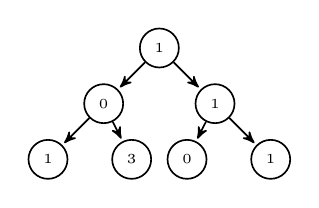
\begin{tikzpicture}[->,>=stealth',shorten >=1pt,auto,node distance=1cm,
                    semithick,initial text=]

  \node[circle,draw]   (0)                    {\tiny 1};
  \node[circle,draw]   (1) [below left of=0]  {\tiny 0};
  \node[circle,draw]   (2) [below right of=0] {\tiny 1};
  \node[circle,draw]   (3) [below left of=1]  {\tiny 1};
  \node[circle,draw]   (4) [below right of=1, xshift=-1em] {\tiny 3};
  \node[circle,draw]   (5) [below left of=2, xshift=1em]  {\tiny 0};
  \node[circle,draw]   (6) [below right of=2] {\tiny 1};
  
  \path (0) edge              node {} (1)
        (0) edge              node {} (2)
        (1) edge              node {} (3)
        (1) edge              node {} (4)
        (2) edge              node {} (5)
        (2) edge              node {} (6);
\end{tikzpicture}
\end{center}
\paragraph{Part (a).} {\bf Write down} an input {\tt choices} that ensures statement coverage when used
together with the above tree.

\paragraph{Part (b).} Assume that you have a single test case which takes the same tree as above.
You can't look at the value of \texttt{choices}. When executed, this case produces output ``1 0 1''.
For each labelled statement {\tt A-G}, {\bf write down} what you know about whether
that statement was reached on this input (definitely reached; definitely not reached;
don't know) and why you know it.

\newpage
\section*{Question 7: Mutation}

Propose two distinct non-stillborn and non-equivalent mutants for the
following method. {\bf Describe} the mutation operator that you used and where you
apply it. Show that you can kill the mutants, demonstrating that they
are non-equivalent mutants, by {\bf writing down} test cases and relevant
outputs for each of these mutants and the original method.

\begin{lstlisting}
public static int odd(int[] x)
// Effects: if x == null, throw NullPointerException
// else: return the number of elements in x that are odd
{
  int count = 0;
  for (int i = 0; i < x.length; i++) {
    if (x[i]%2==1 || x[i]%2==-1) {
      count++;
    }
  }
  
  return count;
}
\end{lstlisting}

\end{document}
